% This is a simple sample document.  For more complicated documents take a look in the exercise tab. Note that everything that comes after a % symbol is treated as comment and ignored when the code is compiled.

\documentclass[11pt]{article} % \documentclass{} is the first command in any LaTeX code.  It is used to define what kind of document you are creating such as an article or a book, and begins the document preamble
\usepackage{amssymb}
\usepackage[utf8]{inputenc}
\usepackage{glossaries}


\makeglossaries

\newglossaryentry{SolCor}{
	name={couronne solaire},
	description={la partie externe de l'atmosphère du soleil, s'étendant sur plusieurs fois le rayon du soleil}
}

\newglossaryentry{SolVoil}{
	name={voile solaire},
	description={une méthode de propulsion experimentale utilisant la pression solaire pour avancer, genère des forces extremement faibles mais ne coûte pas de carburant}
}

\newglossaryentry{Elec}{
	name={moteur ionique},
	description={un moteur fusée propulsant de petites quantités de matières à très grande vitesses à l'aide d'électricité générant ainsi des poussées très faibles mais très efficaces (peu coûteuses en carburant)}
}


\newglossaryentry{Zone}{
	name={zone d'observation},
	description={région dans laquelle le soleil est intégrallement caché pas l'astre occultant mais où l'intégralité de la couronne (avec une certaine tolérance sur les parties les plus proches de la surface) est visible, ici l'astre occultant sera toujours la Lune}
}

\newglossaryentry{Obs}{
	name={observation},
	description={correspond à une trajectoire passive (sans contrôle) durant laquelle l'objet se situe dans la zone d'observation, une observation commence lorsque l'objet entre dans la zone et s'arrête quand il en sort}
}

\newglossaryentry{AscObs}{
	name={observation ascendante},
	description={observation type assez longue ayant lieu entre le premier croissant et le premier quartier de la Lune, durant l'observation l'objet s'éloigne de la Terre.}
}

\newglossaryentry{DesObs}{
	name={observation descendante},
	description={observation type assez longue ayant lieu entre le dernier quartier et le dernier croissant de la Lune, durant l'observation l'objet se rapproche de la Terre.}
}


\newglossaryentry{Cont}{
	name={contrôle},
	description={dans un problème de contrôle optimal le contrôle est une fonction qui dépend de l'état et du temps qui influence la dynamique d'un système, dans le cadre de ce stage, le contrôle est une fonction qui indique un vecteur 3D en fonction du temps correspondant à la poussée du satellite}
}

\newglossaryentry{Cor}{
	name={coronographe},
	description={un téléscope équipé d'un disque opaque cachant la partie la plus lumineuse de l'objet observé permettant d'observer les détails les moins lumineux, utilisé majoritairement pour observer la couronne solaire d'où son nom}
}

\newglossaryentry{SynPeriod}{
	name={periode synodique},
	description={la periode synodique d'une lune correspond au temps nécessaire pour que les trois astres (lune, planète et étoile) retrouve la même position relative, cette periode peut être légèrement plus courte ou plus longue que la vraie periode de la lune à cause du mouvement de la planète autour de l'étoile}
}


\usepackage{amsmath} % \usepackage is a command that allows you to add functionality to your LaTeX code
\usepackage[left=2cm, right=2cm,bottom=2.5cm]{geometry}
\title{Rapport de Stage} % Sets article title
\author{Vincent Callegari} % Sets authors name
\date{\today} % Sets date for date compiled
\usepackage{graphicx}


\usepackage{float}








\graphicspath{{./images/graph/}}
% The preamble ends with the command \begin{document}
	\begin{document}
		\maketitle
		\hspace*{-0.1375\textwidth}
		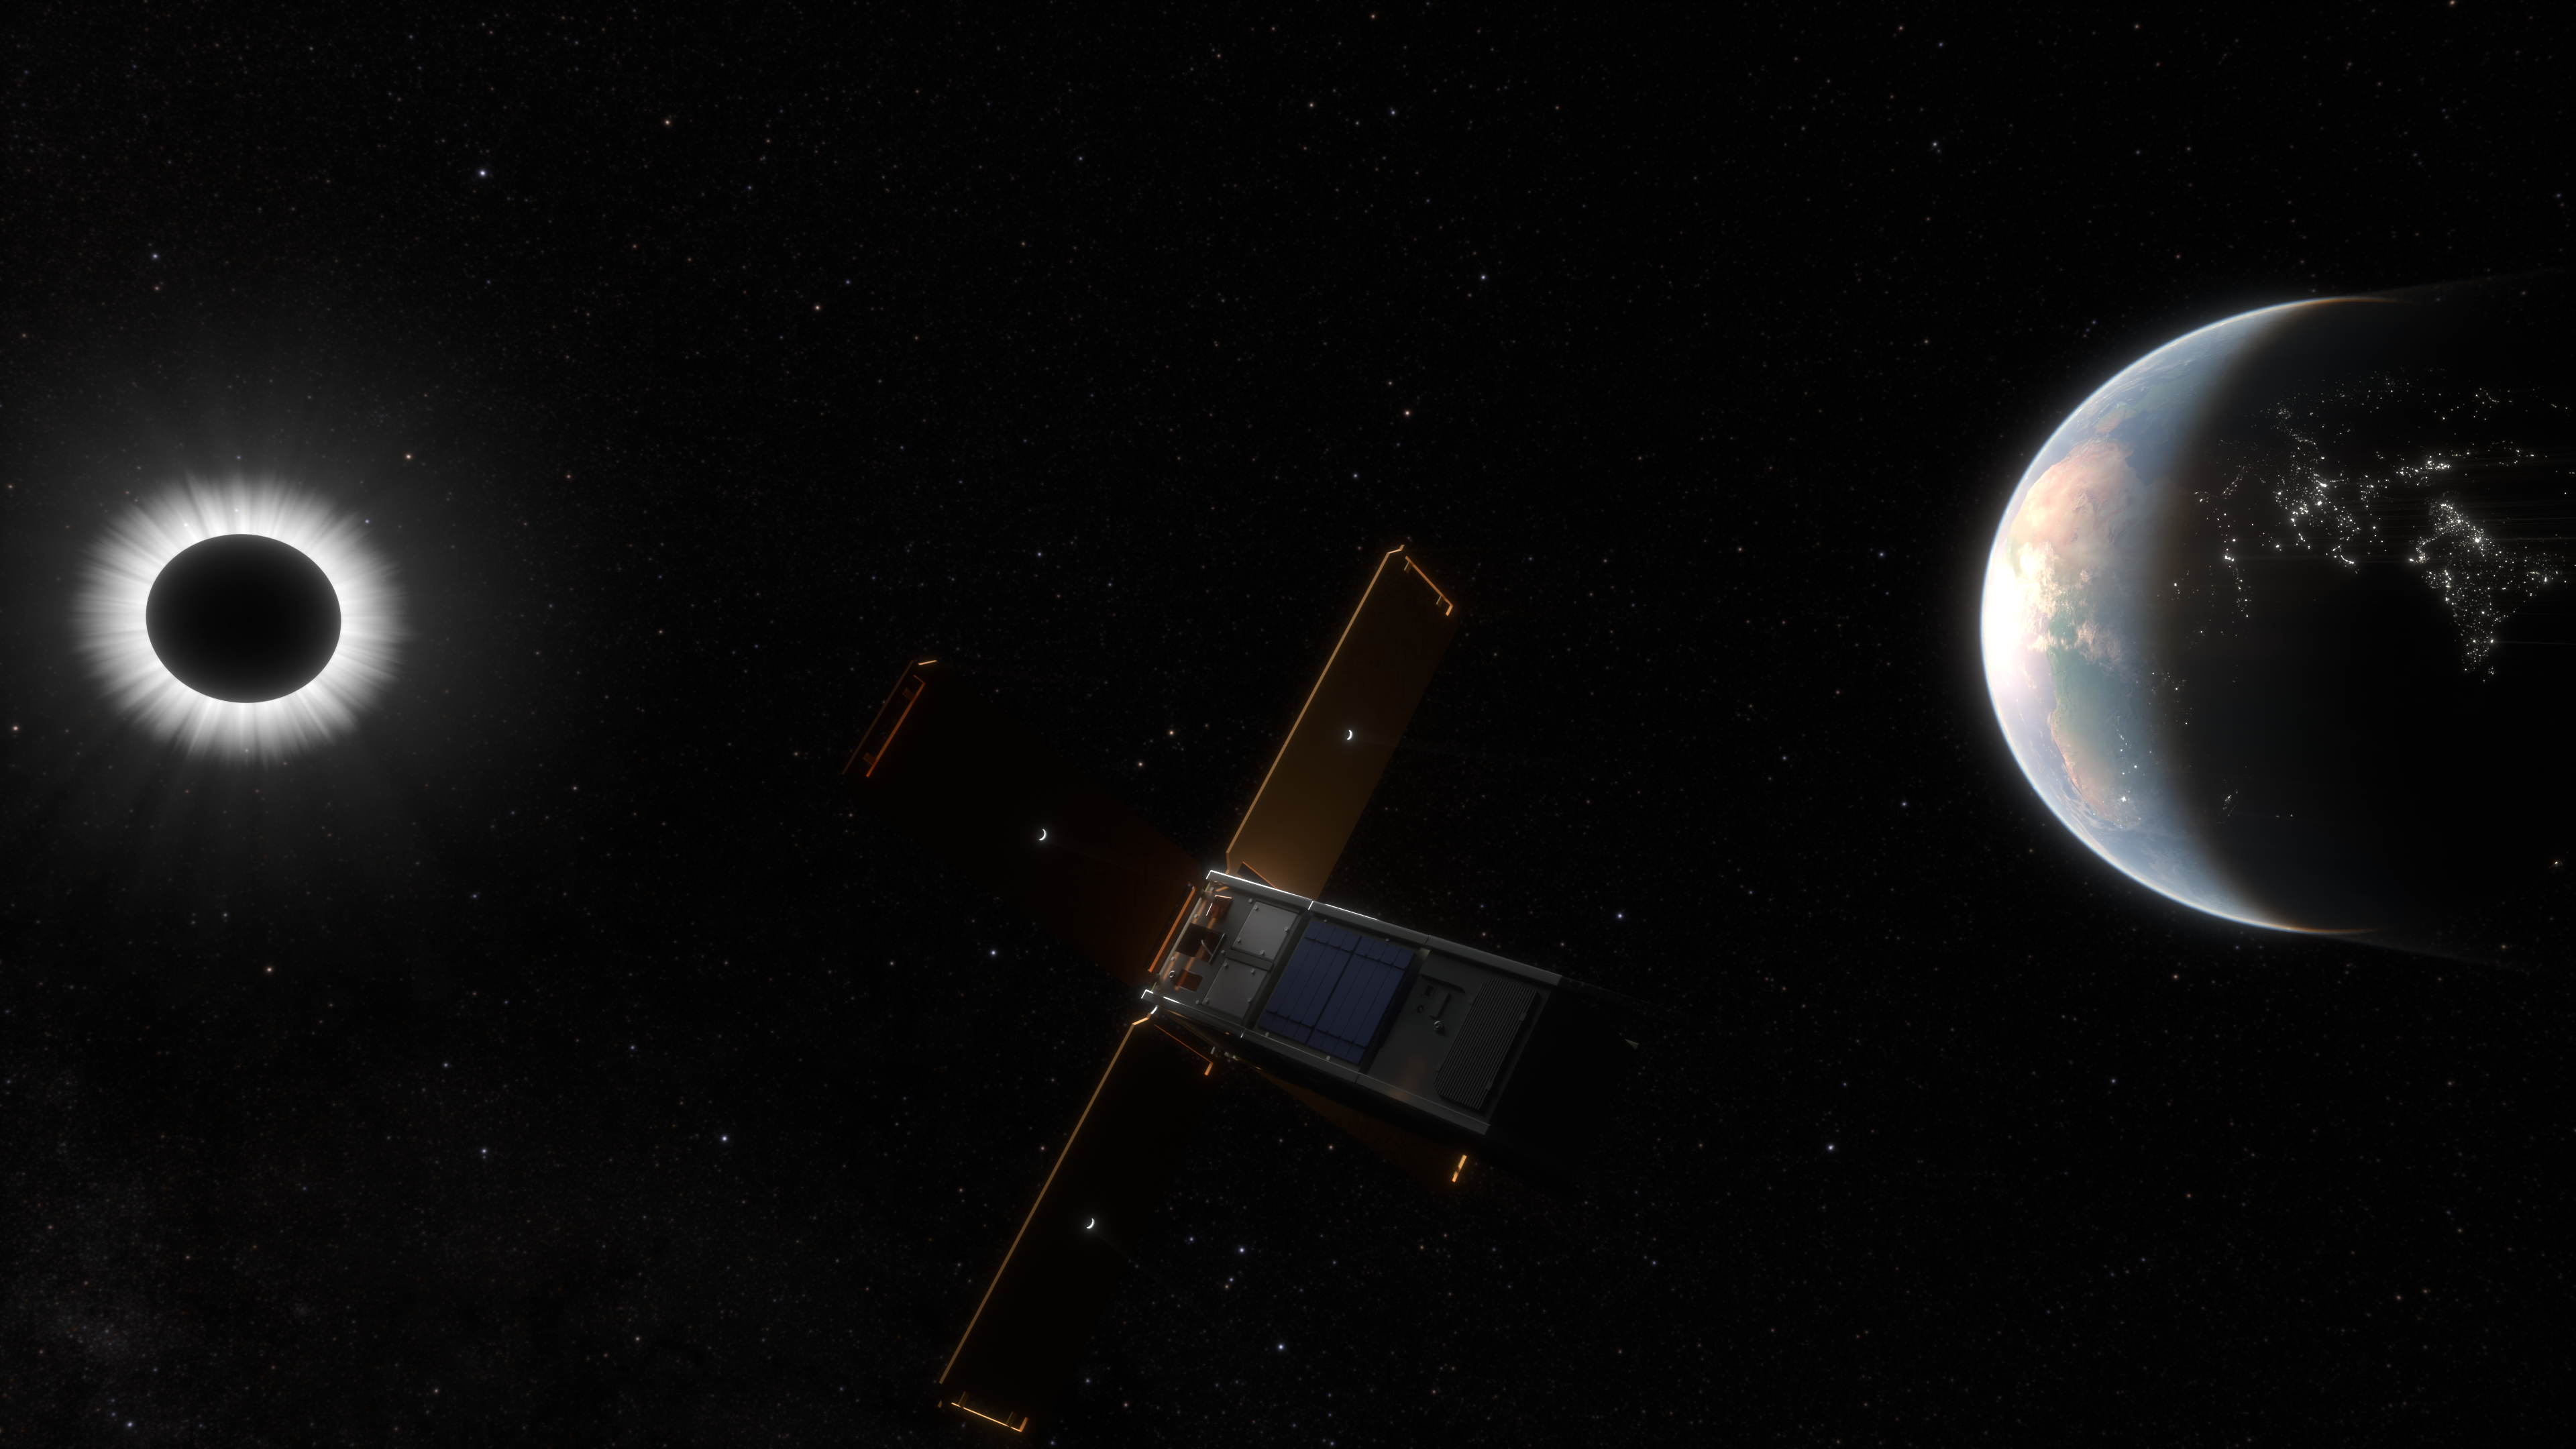
\includegraphics[width=1.2\textwidth]{images/eclipse_3_bis.png}
		\vfill
		\includegraphics[width=3cm]{images/Logo_Reseau_Polytech.png} \hfill \includegraphics[width=3cm]{images/inria.png}
		\newpage
		\tableofcontents
		\newpage
		\section{Introduction}
		
		\subsection{La problématique}
		Le but de ce stage est d'analyser une mission spatiale visant à étudier la \gls{SolCor} en utilisant la Lune comme corps occultant. En outre l'objectif est de calculer des trajectoires optimales faisables par des satellites exerçant des poussées faibles (par \gls{Elec} ou \gls{SolVoil}).
		
		La voile solaire fonctionne de la même manière qu'une voile normale à l'exception qu'elle utilise la quantité de mouvement de la lumière au lieu de la quantité de mouvement de l'air pour générer une force de pression. Les forces générées par des voiles solaires ne peuvent pas être dirigées dans toutes les directions (la force ne peut pas être en direction du Soleil) et sont très faibles en comparaison d'autres formes de propulsions les plus utilisés par les véhicules spatiaux mais ont le grand avantage de ne pas dépendre du carburant.
		
		La propulsion électrique quant à elle utilise un champ magnétique pour accélérer un gaz ionisé (souvent un gaz noble comme le xénon par exemple). L'idée est de créer une propulsion extrêmement efficace grâce à la vitesse très élevée des particules permettant ainsi de faire gagner une grande vitesse au satellite pour une masse de carburant relativement faible. Le désavantage de cette méthode de propulsion est qu'elle ne permet pas de générer de grandes forces de poussée ce qui signifie qu'elle ne peut pas être utilisée avec des vaisseaux trop lourds ou pour le décollage de fusée.
		
		La couronne solaire est en quelque sorte l'atmosphère du soleil, c'est une des parties du soleil qui est la plus mal comprise, on sait que c'est ici que se manifestent des événements violents comme les éruptions solaires ce qui influence la climat terrestre. Notamment les vents solaires peuvent faire varier la densité de l'atmosphère terrestre en haute altitude ce qui impacte les satellites en orbite basse. Essayer de mieux comprendre le fonctionnement de la couronne solaire est donc un objectif assez important des astronomes.
		
		L'observation de la couronne solaire est un tâche difficile car elle est bien moins lumineuse que le soleil lui même. Afin d'observer cette couronne, il est donc nécessaire d'occulter le disque solaire.
		
		Sur Terre il est possible d'effectuer des observations de la couronne solaire durant les éclipses totales où la Lune joue le rôle d'objet occultant. Cependant ces observations ont lieu en moyenne une fois tout les 18 mois et ne permettent que des observations de quelques minutes à peine ce qui n'est pas suffisant.
		
		Une autre méthode pour effectuer de telles observations est d'utiliser un \gls{Cor} qui se sert d'un masque pour cacher la partie la plus lumineuse du Soleil. Cependant, plus l'objet utilisé pour occulter le Soleil est grand et éloigné, plus l'observation peut être précise. Les planètes, planètes naines et autres astres sphériques opaques sont donc des objets idéaux pour effectuer des mesures car leur taille excède largement tout objets occultant que l'humanité peut construire à ce jour. De plus, comme c'est souvent le cas en astronomie, l'atmosphère terrestre ajoute des perturbations lorsque l'on effectue des observations à la surface de la Terre, donc l'observation de la couronne solaire est bien plus efficace depuis l'espace.
		
		L'objet du système solaire qui semble le plus indiqué pour être utilisé comme astre occultant est la Lune car son absence d'atmosphère et sa grande proximité avec la Terre combinés à sa petite taille permettent d'effectuer des observations à distance relativement faible (environ égale à la distance Terre-Lune) tout en ayant les avantages énoncés plus tôt.
		 
		La contrepartie lorsque l'on utilise une astre comme objet occultant est qu'on ne peut contrôler sa trajectoire et que le satellite est contraint de suivre l'objet, ce qui demande de résoudre un certain nombre de problèmes et de se plier à un certain nombre de contraintes.
		
		Ainsi l'objectif de mon stage est d'étudier les possibilités d'effectuer des observations de la couronne solaire en utilisant la Lune comme objet occultant.
		 
		Dans ce rapport, je vais détailler le travail que j'ai effectué et les conclusions et résultats auxquels je suis arrivé ainsi que les compétences acquises au cours du stage. 
		 
		\subsection{Institut de recherche}
		
		l'Institut national de recherche en informatique et en automatique (INRIA) est un laboratoire public de recherche. Il est implémenté sur nombreux sites :  Bordeaux, Grenoble, Lille, Lyon, Lorraine, Paris, Rennes, Saclay, Côte d'Azur et le Chesnay. J'ai effectué mon stage sur le site de Sophia Antipolis (Alpes Maritimes). Le laboratoire à été fondée en 1967 (il s'appelait alors seulement l'Institut de recherche en informatique et en automatique ou IRIA) dans le cadre de l'initiative du plan Calcul visant à s'assurer que la France conserve une indépendance en innovation informatique.
		
		J'ai effectué mon stage au sein de l'équipe McTao qui est une équipe qui développe des méthodes de contrôle optimal dans des systèmes non linéaires.
		
		\section{Travail demandé}
		\subsection{Objectif du stage}
		Le travail qui m'a été demandé durant ce stage regroupait plusieurs tâches : tout d'abord, étudier la géométrie de la \gls{Zone} au cours du temps (la zone d'observation étant la région où le soleil est caché par la lune mais où la couronne solaire reste visible). Ensuite il fallait, à partir de ces résultats, essayer de trouver des trajectoires permettant de traverser la zone d'observation de manière répétée et ensuite de maximiser le temps d'observation.
		
		Plusieurs corps célestes seront pris en compte dans l'étude de ce problème : Le Soleil, La Terre et la Lune. Il s'agit donc d'un problème à quatre corps (les trois énoncés plus tôt en plus du satellite). En physique un problème à n corps est un problème de dynamique dans lequel n corps sont pris en compte, chacun exerçant sur les autres des forces de gravité telles qu'elles sont décrites par Newton. Dans ce contexte il est presque impossible de trouver une trajectoire passive (sans \gls{Cont}) permettant de faire des observations répétées (un problème de plus de 2 corps ne permet pas des orbites cycliques). Ainsi il est nécessaire d'ajouter un contrôle au système c'est à dire ajouter un système de propulsion au satellite pour lui permettre de modifier sa trajectoire. Il était initialement prévu d'utiliser une \gls{SolVoil} comme méthode de propulsion mais il s'avérera plus pratique d'utiliser un \gls{Elec}.
			
		%Étant donné qu'il y aura sans doute de nombreuses forces perturbatrices et qu'une trajectoire passive (un objet sans contrôle qui ne subit que les forces de gravité de la Terre, Lune, Soleil etc ...) ne traversera sans doute pas la zone d'observation très souvent, il est nécessaire d'ajouter au système un contrôle pour corriger la trajectoire du satellite voire de la changer. le système de propulsion qui à été choisi pour accomplir cet objectif est une voile solaire. Il s'agit d'un problème de contrôle optimal ce qui signifie que j'ai du en apprendre plus sur dans ce domaine car je n'ai pas encore suivi les cours sur ce sujet.
		
		Le but final du projet est de présenter un rapport rapportant tous les résultats et observations faits lors du stage ainsi que des programmes capables de calculer différentes valeurs utiles (zone d'observation, trajectoire de satellite ou contrôle de ce dernier).
		\subsection{Tâches}
		En résumé mon travail se répartit en plusieurs étapes décrites ci après:
		\begin{itemize}
			\item Calculer la géométrie de la \gls{Zone};
			\item Trouver des trajectoires passives (sans contrôle) qui permettent des \glspl{Obs};
			\item Trouver des trajectoires actives (avec contrôle) qui permettent des observations répétées;
			\item Résumer tous les résultats dans un rapport en anglais.
		\end{itemize}
		
		Calculer la dynamique de la \gls{Zone} demande dans un premier temps d'étudier de la littérature scientifique en rapport avec ce sujet. Il faut ensuite mettre au point un bon modèle mathématique pour définir la géométrie de la zone d'observation ainsi qu'un modèle pour son déplacement. Pour cela il faudra trouver une méthode qui permet de déterminer si un objet est dans la zone d'observation.
		\\ \\
		L'étape suivante consiste à trouver des trajectoires passives (c'est à dire sans \gls{Cont}) traversant la zone d'observation. Pour cela il faut implémenter un programme qui simule la dynamique de l'objet ainsi qu'une méthode adaptée pour évaluer des trajectoires qui permettent des observations. Cette étape permettra de déterminer la forme générale  des \glspl{Obs} intéressantes ce qui sera utile pour l'étape suivante.
		\\ \\
		Par la suite il faut ajouter un contrôle dans l'optique de maximiser le nombre d'observations. On utilisera la toolBox OptimalControl.jl développer en Julia
		\\ \\
		Pour finir il faut résumer tout le travail et tous les résultats obtenus dans un rapport rédigé en anglais ainsi que rendre les programmes informatiques produits lisibles et clairs pour le développement ultérieur du projet
		\\ \\
		%De plus le modèle utilisé pour résoudre ce problème sera d'abord implémenté dans une version simplifiée : simple trajectoire circulaire de la lune avec vitesse fixe en 2D. Puis gagneras en complexité au fur et à mesure que le projet avanceras jusqu'à être très proche de la réalité (prise en compte de la variation de l'orbite lunaire causé par le soleil par exemple).
		
		\section{Travail effectué}
		
		\subsection{Analyse de la zone d'observation}
		Avant de commencer à travailler sur le problème, il fallait que j'en apprenne plus sur les notions du projet, j'ai donc lu divers articles qui m'ont été fournis:
		
		\begin{itemize}
			\item Un article sur une mission d'occultation solaire avec la Terre : Trajectory design of Earth-enabled Sun occultation missions |Nicolò Bernardini, Nicola Baresi, Roberto Armellin, Steve Eckersley, Sarah A. Matthews | 2022
			\item une thèse sur les voiles solaires : Contrôle optimal des voiles solaires | Alesia Herasimenka | 2023
			\item un cours sur la mécanique spatiale : An Introduction to the 
			Mathematics and Methods of 
			Astrodynamics, Revised Edition | Richard H. Battin | 1999 
			\item un cours sur le contrôle optimal : An Introduction to Mathematical
			Optimal Control Theory | Lawrence C. Evans | 2008
		\end{itemize}
		
		% Il y avait des articles sur des projets d'occultation solaire à l'aide de la Terre (utilisée comme astre occultant), une thèse sur les voiles solaires, ainsi qu'un cours sur le contrôle optimal car je n'ai pas encore eu de cours sur ce sujet.
		
		J'ai ensuite analysé le déplacement de la \gls{Zone} de la Lune. J'ai utilisé des notions basiques de géométrie pour déterminer où se trouvait la zone d'observation de la Lune en fonction de la position de cette dernière.
		
		La forme de la zone d'observation dépend de la taille de l'objet occultant ($R_l$) et du Soleil ($R_s$), de la distance entre le Soleil et l'objet (ici environ la distance Terre-Soleil soit environ 150 millions de km) ainsi que de la précision de l'observation. En effet plus on souhaite observer des parties de la couronne proche du soleil plus la zone d'observation sera réduite car il faudra être plus proche du point où le Soleil est exactement caché par l'astre occultant sans que cet astre cache la zone périphérique du soleil. Cette valeur est définie par un pourcentage du rayon solaire appelé $\alpha$, une valeur de $\alpha$ de $5\%$ par exemple signifie que l'on tolère que des parties de la couronne solaire étant à moins de $0.05$ rayon solaire de la surface de celui ci soit cachées par l'astre occultant.
		
		La forme de la zone d'observation est l'intersection de deux cônes : le cône dans lequel la couronne solaire est visible (en prenant en compte la tolérance $\alpha$) et le cône dans lequel le soleil est caché.
		
		\begin{figure}[H]
			\includegraphics[width=0.9\textwidth]{images/moon_schem.png}
			\caption{Géométrie de la zone d'observation}
		\end{figure}
		
		J'ai obtenu les formules suivantes pour les positions des points $P_1$, $P_2$ et $P_3$ relativement à la Lune quand elle est à une distance $D$ du Soleil comme illustré dans la figure 1. On part également du principe que la Lune et le Soleil sont alignés le long de l'axe X.
		
		$$	
		P_{1x}=\frac{\bar{D}R_l}{R_s-R_l}
		$$ 
		$$	
		P_{3x}=\frac{\bar{D}R_l}{R_s(\alpha+1)-R_l}
		$$
		$$
		P_{2x}=\frac{P_{1x}\tan(\theta_1) + P_{3x}\tan(\theta_3)}{\tan(\theta_1) + \tan(\theta_3)}
		$$
		$$
		P_{2y}=\tan(\theta_1)(P_{1x}-P_{2x})
		$$
		
		avec
		$$
		\theta_1=\sin^{-1}\left(\frac{R_l}{P_{1x}}\right)
		$$
		
		$$
		\theta_3=\sin^{-1}\left(\frac{R_l}{P_{3x}}\right)
		$$
		
		Afin d'économiser de la puissance de calcul, il est possible de ne pas avoir à recalculer de nouveau la position des points $P_1$ et $P_3$ si on connait leur position en fixant la Lune à une position de référence (on appelle les points quand la Lune est dans cette position de référence $\hat{P}_1$ et $\hat{P}_3$). 
		
		A partir de ces valeurs il est possible de déterminer les positions exactes des points $P_1$ et $P_3$ quelle que soit la position de la Lune à l'aide d'un simple produit en croix:
		
		$$
			P_3=r_{l}+\hat{P}_{3x}D^{-1}r_{ls} 
		$$
		$$
			P_1=r_{l}+\hat{P}_{1x}D^{-1}r_{ls}
		$$
		
		Ici $r_{l}$ et $r_{ls}$ correspondent respectivement à la position de la Lune et la position de la Lune relativement au Soleil tandis que $D$ représente la distance Soleil Lune quand la Lune est à sa position de référence .
		
		La position réelle du point $P_2$ est approximée pour ne pas avoir à recalculer les angles $\theta_1$ et $\theta_3$. J'ai choisi d'utiliser cette méthode approchée pour évaluer la zone d'observation pour essayer de réduire le coût de calcul. Cela permettra d'accélérer l'exécution du code qui sera implémenté plus tard car cette opération sera répétée extrêmement souvent.
		
		En prenant $D$ égal à la distance Terre soleil, j'ai calculé qu'on obtient une erreur de l'ordre de quelques centimètres sur la position du point $P_{2y}$ ce qui est négligeable en comparaison de l'épaisseur de la zone d'observation.
		
		Pour une valeur de $\alpha$ de $5\%$ la zone d'observation à une longueur d'environ $18000$ km pour une épaisseur d'environ $85$ km. On peut ainsi voir que la zone d'observation est extrêmement fine.
		
		Après avoir utilisé des outils graphiques pour visualiser clairement la forme de la \gls{Zone} et avoir déjà calculé à la main des candidats d'\gls{Obs} qui semblaient être intéressantes.
		
		Concernant la dynamique du système les états (positions et vitesses) de la Terre et de la Lune sont calculés avant de calculer la trajectoire du satellite dans un système à trois corps avec le Soleil fixé à l'origine. On peut faire le calcul ainsi car on néglige l'influence du satellite sur la trajectoire des trois astres car la masse de ce dernier est ridiculement faible en comparaison des autres objets du système. De cette manière on n'aura besoin de résoudre uniquement un problème à trois corps au lieu de quatre et surtout une unique fois au début du calcul au lieu d'une fois à chaque fois que l'on veut calculer la trajectoire du satellite. Une fois ce système résolu la dynamique du satellite est calculée avec les équations suivantes dans le référentiel du centre de gravité du système Terre-Lune :
		
		$$
		\begin{bmatrix}
			\dot{\overrightarrow{r_{s}}}\\
			\dot{\overrightarrow{v_{s}}}\\
		\end{bmatrix} =\begin{bmatrix}
			\overrightarrow{V_{s}}\\
			G_{m}(r_s,r_l)+G_{t}(r_s,r_t)
		\end{bmatrix}
		$$
		
		avec $G_m$ et $G_t$ respectivement la force de gravité lunaire et la force de gravité terrestre. Notez que la gravité solaire ne figure pas dans l'équation car on se place dans le référentiel du système Terre-Lune (bien qu'il faudrait techniquement prendre en compte la très légère variation de la force de gravité solaire). Dans cette équation le satellite n'a pas de contrôle car il ne peut pas à la fois observer et changer sa trajectoire.%modif
		
		\subsection{Calcul du temps d'observation}
		Ensuite J'ai implémenté le modèle dans Matlab ainsi qu'une méthode permettant de calculer le temps passé dans la \gls{Zone} en fonction de la vitesse et la position initiale du satellite situé dans la zone d'observation. De par la longueur importante la zone d'observation, j'ai choisi de simplifier l'ensemble des positions initiales possibles du satellite par une ligne reliant les points $P_1$ et $P_3$. La méthode permettant de calculer le temps passé dans la zone d'observation simule la dynamique du système jusqu'à ce que le satellite sorte de la zone puis simule la dynamique en sens inverse pour remonter jusqu'au moment où le satellite est entré dans la zone. Les temps d'entrée et de sortie de la zone d'observation permettent de calculer le temps passé dans la zone d'observation. L'objectif du problème est de maximiser le temps passé dans la zone d'observation. Avec ce modèle on ne considère que les trajectoires qui n'effectuent qu'une seule observation (ou alors si elles en font plusieurs on n'en considère qu'une seule). Ce choix à été fait car j'ai remarqué qu'il y avait quelques points précis qui permettaient des temps d'observation extrêmement longs (plus de 15 heures) par rapport aux temps d'observation médians (quelques minutes). Je suis donc arrivé à la conclusion qu'il serait sans doute inutile de chercher des orbites permettant plusieurs observations quand une trajectoire effectuant une seule de ces longues observations serait meilleure en tous points.
		\\ \\
		J'ai pu obtenir des premiers résultats consistant simplement, pour chaque paramètre, à le laisser libre pendant que l'on fixait tous les autres puis à afficher dans un graphe la variation du temps d'observation en fonction du paramètre laissé libre. Ces résultats ont permis de mettre en évidence deux points de l'orbite lunaire qui semblaient être assez intéressants pour effectuer de longues observations : ces deux points se situent aux moments où le Soleil, la Terre et la Lune forment un angle d'environ 60 degrés (j'ai nommé ces observations \gls{AscObs} et \gls{DesObs}). Du point de vue de la Terre cela représente les moments où un tiers de la Lune est illuminé par le Soleil (entre le premier croissant et premier quartier par exemple).Pour effectuer une observation le satellite doit se situer également sur l'orbite lunaire mais 60 degrés plus loin (le Soleil, la Terre et le satellite formeraient donc un angle de 120 degrés) mais se déplacerait dans la même direction que la Lune afin d'accompagner la zone d'observation, ces observations sont illustrées dans la figure 2. Il faut noter cependant que ces résultats sont valables uniquement dans un modèle très simplifié vérifiant les hypothèses suivantes :
		\begin{itemize}
			\item orbite de la Lune sans variation (keplerienne) et parfaitement circulaire;
			\item Soleil fixé;
			\item forces de gravité de la Lune sur le satellite négligées;
			\item distance entre la Lune et la zone d'observation fixée à la distance Terre Lune.
		\end{itemize}
		
		\begin{figure}[h]
			\includegraphics[width=18cm]{images/observations_main.png}
			\caption{orbites kepleriennes qui permettent de faire des observations particulièrement longues, ces observations sont plus longues car la vitesse du satellite et de la zone d'observation sont similaire.}
		\end{figure}
		Au fur et à mesure que le projet a avancé, j'ai amélioré le modèle en prenant en compte de plus en plus de facteurs comme l'excentricité et l'inclinaison de l'orbite de la Lune, la gravité de la Lune qui influence la dynamique du satellite ainsi que les variations de l'orbite de la Lune et de la Terre causées par l'influence gravitationnelle du Soleil sur le système Terre Lune (voir figure 3). Les trajectoires intéressantes qui ont été décrites plus tôt sont restés les meilleures trajectoires possibles bien qu'elles n'aient plus lieu exactement au mêmes endroits à cause des nouveaux facteurs du problème.
		\begin{figure}[h]
			\includegraphics[width=1\textwidth]{images/moon_orbit.jpg}
			\caption{variation de l'orbite lunaire sur 2 ans}
		\end{figure}
		
		Aux termes du projet, le code MATLAB que j'ai réalisé avait d'une longueur d'environ 600 lignes et effectuait plusieurs opérations qui sont listées ci dessous: 
		
		\begin{itemize}
			\item Simuler la dynamique du système à trois corps Soleil Lune Terre (l'influence du système Terre-Lune sur le soleil est négligé);
			\item obtenir des approximations des emplacements des \glspl{Obs} optimales dans le but de trouver de bonnes conditions initiales à l'aide d'un modèle simplifié;
			\item optimiser les observations optimales pour chaque minimum trouvé à l'étape précédente;
			\item obtenir des images graphiques et des fichiers csv contenant les données.
		\end{itemize}
		
		Le code a besoin en entrée de multiples informations sur la dynamique du problème dont la plupart des facteurs sont fournis directement dans le code. La partie venant de l'extérieur du code sont les positions et vitesses initiales du soleil de la Lune et de La Terre ainsi que quelques informations sur le nombre d'observations qu'il faut récupérer.
		Ce code pourrait être facilement adapté en une librairie qui pourra être ensuite incorporée dans des outils plus avancés par d'autres utilisateurs.
		Ce travail permis de confirmer l'intérêt des deux points de l'orbite lunaire qui semblaient être les plus intéressants avec des temps d'observation situé entre 15 et 25 heures. En sachant qu'il y a deux observations de ce type pour chaque \gls{SynPeriod} lunaire (environ 29.53 jours), cela permettrait de faire des observations pendant environs 2.8\% du temps (ou 1.4\% du temps en n'en faisant qu'une sur deux) de la mission ce qui est bien mieux que ce que l'on peut faire sur Terre (une observation de 10 minutes tout les 18 mois en moyenne soit environ 0.0015\% du temps).
		
		Le fait que les temps d'observation soient bien plus longs aux points spécifiques où le satellite est lancé depuis la zone d'observation à la même vitesse que cette dernière m'a poussé à faire un test dans lequel le satellite est toujours lancé à la même vitesse que la zone d'observation sans se soucier de sa période. Ce test à bien confirmé que les 2 observations trouvées précédemment sont parmi les plus efficaces mais a permis de mettre en évidence un $3^{eme}$ point de l'orbite lunaire aux alentours de $0^o$ (c-à-d quand le Soleil, la Terre et la Lune sont alignés dans cette ordre). Cependant, cette troisième trajectoire n'est pas idéale car, en plus ne pas avoir une période similaire à celle de la lune, l'observation a lieu à proximité de la zone d'ombre de la Terre ce qui rendrait l'observation impossible si la zone d'observation traversait l'ombre de la Terre. De plus, l'excentricité de l'orbite associée à cette trajectoire est aux alentours de 1 ce qui implique que le satellite pourrait facilement quitter le système Terre Lune ce qui pourrait être un problème en plus d'impliquer une énergie de mise en orbite initiale bien plus importante, c'est pourquoi cette observation n'a pas été étudiée dans l'étape suivante.
		\begin{figure}[h]
			\includegraphics[width=0.9\textwidth]{images/observation_Obs.png}
			\caption{temps d'observation en fonction de la l'angle entre l'axe X et la position de la Lune. La Terre est à l'origine et le soleil se situe à environ -150 million de km le long de l'axe X.}
		\end{figure}
		
		
		\subsection{Contrôle optimal}
		
		L'étape suivante consiste à calculer la trajectoire du satellite pour joindre les différentes observations.
		pour cela j'ai utilisé une librairie en Julia permettant de résoudre des problèmes de contrôle optimal, l'idée était de calculer tous les transferts possibles entre différentes observations.
		
		On utilise la même méthode que précédemment pour calculer la position de la Terre et de la Lune, cependant on ajoute un contrôle à la dynamique du satellite ainsi qu'un paramètre supplémentaire pour la masse :
		
		L'état initial du satellite est fixé et l'état final l'est également à l'exception de la masse qui est laissée libre (mais contrainte supérieure à la masse du chargement du satellite). Les temps de départ et d'arrivée sont également fixés.
		L'objectif est de minimiser le contrôle. Pour cela on définit le problème de contrôle optimal suivant :
		
		$$
		\dot{x}=
		\begin{bmatrix}
			\dot{\overrightarrow{R_{s}}}\\
			\dot{\overrightarrow{V_{s}}}\\
			\dot{m_{s}}
		\end{bmatrix} =\begin{bmatrix}
			\overrightarrow{V_{s}}\\
			G_{m}(R_s,R_m)+G_{t}(R_s,R_t)+u\frac{M_{t}}{m}\\
			-Q\|u\|
		\end{bmatrix}
		$$
		$$
			x(t_0)=\begin{bmatrix}
				r_0\\
				v_0\\
				m_i
			\end{bmatrix}
		$$
		$$
		x(t_f)=\begin{bmatrix}
			r_f\\
			v_f\\
			m_f
		\end{bmatrix}
		$$
		$\min_{u}C=\int_{t_0}^{t_f}\frac{1}{2}\|u\|^2dt$
		
		Voici ci dessous quelques schémas illustrant les liens entres les orbites de départ et d'arrivée étudiés, le transfert entre une observation descendante à ascendante (en haut à droite) demande de trop grands changements d'orbite en un temps trop court (environ 10 jours) le rendant infaisable. Le passage d'une observation descendante à une observation ascendante en sautant un mois (en bas à gauche) est très facile car les orbites se retrouvent quasiment alignées et laissent plus de temps pour effectuer le transfert (environ 40 jours). Cependant le transfert inverse (en bas à droite) demande au contraire plus d'énergie car les orbites se sont encore plus éloignées au lieu de se rapprocher. De manière générale les transferts entre deux observations du même type demande une quantité relativement faible d'énergie.
		\begin{figure}[H]
			\centering
			\includegraphics[width=0.45\textwidth]{images/1in2obs.png}
			\includegraphics[width=0.45\textwidth]{images/odd_to_even.png}
			\includegraphics[width=0.45\textwidth]{images/1in3_obs.png}
			\includegraphics[width=0.45\textwidth]{images/1in3_bad.png}
		\end{figure}
		
		Les accélérations maximales nécessaires pour ces transferts (de l'ordre de $10^{-4}$ m/s²) se sont avérées trop élevées pour des voiles solaires (qui ne peuvent délivrer que des accélérations de l'ordre de $10^{-5}$ m/s²), c'est à partir de ce moment-là que l'option des voiles solaires a été écartée au profit des moteurs ioniques.	
		%Après avoir implémenté une version simplifiée du problème des voiles solaires (poussée faible dans n'importe quelle direction), il se trouve que les accélérations demandées semblaient trop élevées pour utiliser une voile solaire, l'option d'utiliser un satellite à poussée faible a donc été sélectionné.
		
		Concernant les transferts, j'ai effectué une analyse des résultats qui m'ont permis de sélectionner 2 scénarios possibles de mission dans lesquels un satellite effectue une observation sur 2 en utilisant une poussée faible.
		
		Suite à ces premiers calculs j'ai utilisé comme moteur d'exemple le RIT-10 evo, qui est un moteur développé par le groupe Ariane, ce moteur délivre une force d'environ 0.025 Newton avec une impulsion spécifique d'environ 3000s, cela représente une consommation de carburant de l'ordre de 3 grammes par heure. Le module de test utilisé a une masse totale de 90 kg dont 40 sont du carburant. Ce nouveau code a ensuite été raffiné pour effectuer les opérations suivantes : 
		
		\begin{itemize}
			\item simuler la dynamique du système à trois corps Soleil Lune Terre (l'influence de du système Terre-Lune sur le soleil est négligé);
			\item définir et résoudre un modèle de contrôle optimal de transfert avec bord fixé en minimisant l'énergie dépensée pour chaque transferts des deux scénarios sélectionné.
			\item écrire les résultats dans des fichiers csv.
		\end{itemize}
		\subsection{Analyse des résultats}
		
		Pour finir j'ai du rédiger un rapport (pas ce rapport-ci) qui résumait ma démarche de recherche en détail. L'objectif est d'utiliser ce rapport pour en faire potentiellement une publication scientifique.
		
		Ce rapport devait être rédigé intégralement en anglais. 
		
		Voici les conclusions auxquelles je suis arrivé et que j'ai consigné dans le rapport: 
		
		Concernant les observations, il y a trois points de l'orbite lunaire qui permettent des observations de plusieurs heures. Il y a tout d'abord deux observations symétriques se produisant lorsque le Soleil, la Terre et la Lune forment un angle d'environ 60 degrés (observations que j'ai appelées \gls{AscObs} et \gls{DesObs}). Ensuite il y a également une observation se produisant lorsque le Soleil, la Terre et la Lune sont alignés. Cette dernière observation à été écartée car elle présentait des désavantages par rapport aux deux autres bien qu'elle semble permettre des observations plus longues de quelques heures.
		
		Concernant les changements de trajectoire, il semble que la quantité d'énergie nécessaire pour effectuer un transfert soit proportionnelle au décalage  les orbites associées aux observations. Décalage majoritairement causé par la rotation de la Terre autour du Soleil. Rotation qui augmente à peu près linéairement avec le temps. Cela veut dire la puissance que devra délivrer le satellite sera environ la même quelle que soit la quantité d'observations effectuées (sauf si l'on fait extrêmement peu d'observations).
		
		Par rapport au scénario de mission, il s'est avéré que la puissance nécessaire pour effectuer un nombre satisfaisant d'observations était trop élevée pour une \gls{SolVoil}. Cependant, cette puissance était suffisamment faible pour un \gls{Elec}. C'est ainsi que je suis arrivé à la conclusion d'effectuer une observation sur deux en utilisant un moteur ionique ce qui permettra un mission d'une durée pouvant aller jusqu'à 5 ans en supposant que le carburant est la seule contrainte sur la durée de la mission.
		
		%A plusieurs reprises durant ce stage j'ai du commenter des résultats de calculs, j'ai du rechercher les raisons et les causes qui ont mené à certains résultats inattendus. Pour commencer j'ai utilisé les résultats du solver qui trouvait les plus long temps d'observations pour isoler des les points les plus intéressants  (\gls{AscObs} et \gls{DesObs}) pour faire des observations. Suite à ces analyse j'en ai conclu que ce qui semblait le plus intéressant était d'optimiser les observations indépendamment les unes des autres puis de chercher par la suite des trajectoire de transfert qui permettrait de passer d'une orbite à l'autre.
		
		%J'ai également du faire de choix en fonctions de ces résultat. J'ai par exemple remarqué qu'en prenant une période de révolution plus courte pour le satellite ( de l'ordre de $0.92$ période lunaire au lieu de $1$) les temps d'observation obtenue était plus court. Je pense que la cause de ces résultat vient du fait que la contrainte de vitesse lié à la période fixée du satellite est de trop, cependant donner au satellite la liberté d'avoir n'importe quelle vitesse en partant des optimums trouvé avec le modèle simplifié donne de très mauvais résultat. J'ai donc décidé d'optimiser d'abord avec la norme de vitesse fixé par la période du satellite (fixé à $0.92$) puis de résoudre à nouveau avec un modèle modifié laissant la vitesse libre en prenant comme condition initiale le résultat de l'algorithme précédent. Il est probable qu'il faillent remplacer le modèle simplifié par un autre plus performant. Un qui prendrait en compte le temps d'observation en fixant la vitesse de l'objet à la vitesse de la zone d'observation comme dans la figure 2 par exemple. Mais la forme assez complexe des optimums (deux pics très rapproché) et le fait que les observations des résultats ont rarement montré des trajectoire à vitesse nulle au centre de la zone (les vitesses sont souvent nulles près des bord de la zone) ont fait que je n'ai pas eu le temps d'implémenter un autre modèle.
		
		%Ensuite j'ai du analysé les résultats de mon second code fait en Julia pour essayé de comprendre pourquoi les accélérations maximale des transferts ne diminuait pas même en faisant des transferts sur plus longtemps.
		%Il s'avère que, si l'on considère un modèle simplifié d'une Lune et d'une Terre avec une orbite circulaire sur le même plan, les orbites d'observations sont sensiblement les mêmes avec pour unique différence une rotation autour du vecteur normal au plan écliptique. Cette rotation est proportionnelle aux temps entre deux observation. Cela signifie que plus deux observations sont éloigné plus il faudra faire tourner l'orbite d'observation sur un grand angle ce qui explique que la les accélérations maximales ne diminuaient pas. Effectuer un transfert sur une observation deux fois plus lointaine dans le temps nécessite de faire tourner l'orbite d'observation deux fois plus loin également. C'est cette conclusion suggérant qu'il y a un seuil d'accélérations minimal que doit atteindre le satellite pour effectuer un nombre important d'observations par an qui à mené à l'abandon des voiles solaires au profit d'un moteur à poussée faible.
		
		\begin{figure}[H]
			\centering
			\includegraphics[width=0.9\linewidth]{images/Transfert_23_25}
			\caption{Trajectoire typique suivie par le satellite lors d'un transfert entre deux observations, les lignes rouges symbolisent la force de poussée}
		\end{figure}
		\begin{figure}[H]
			\centering
			\includegraphics[width=0.9\linewidth]{images/All_transfert_even_48_50}
			\caption{L'intégralité des transferts de l'un des deux scénarios possibles pour une mission de 2 ans allant de janvier 2025 à janvier 2027}
		\end{figure}
		\newpage
		\section{Conclusion}
		\subsection{Compétences acquises}
		Pour conclure ce stage m'a permis d'obtenir de nombreuses compétences.
		J'ai eu l'occasion de maîtriser les bases du contrôle optimal. Ce stage m'a également permis de mettre en application ces connaissances en utilisant une librairie permettant de résoudre des problèmes de ce type.
		
		J'ai également renforcé mes compétences en programmation en apprenant un nouveau langage de programmation: le Julia qui est un langage utilisé en recherche pour le calcul scientifique et la résolution numérique de problèmes. J'ai également grandement amélioré mes connaissances dans le langage de programmation Matlab qui est lui aussi un langage utilisé pour la résolution numérique de problèmes.
		
		Le fait de programmer en deux langages différents m'a forcé à faire transiter les résultats d'un programme à l'autre en utilisant des fichiers csv ce qui m'a permis de faire des applications plus propres et à renforcé mes capacités à créer des codes pouvant être inclus et utilisés dans d'autres applications que celles pour lesquelles ils avaient été initialement programmés.
		
		J'ai également eu l'occasion d'écrire un compte-rendu de projet intégralement en Anglais ce qui, en plus de renforcer mes compétences en Anglais, m'a permis de devenir plus doué dans la rédaction de rapports scientifiques en vue de publication.
		
		\subsection{Travail réalisé}
		
		Durant ce stage j'ai produit de nombreux résultats qui pourront être réutilisé par d'autres personnes à l'avenir. 
		\\ \\
		Premièrement j'ai produis deux programmes, un programme réalisé avec le langage MATLAB qui calcule toutes les observations faisables sur un intervalle de temps, ce programme prends en entrée plusieurs fichiers CSV contenant des paramètres sur le code à exécuter nombre d'observation à récupérer,la valeur de alpha etc ...) ainsi que les positions initiales de la Terre la Lune et le Soleil. Ce code produit comme résultat plusieurs fichiers CSV correspondant aux temps de départ et de fin d'observation ainsi que les positions et vitesses qu'aurait un objet effectuant ces observations à l'entrée et la sortie de la zone d'observation.
		
		J'ai également produit un code en Julia qui prend en entrée les résultats du code précédent (dans le même format de fichier) et calcule des trajectoires avec contrôle qui permettent de relier des observations. Ce programme donne en sortie de nombreuses données de résultats sous le format CSV.
		
		Ces deux programmes donnent aussi chacun des graphiques et des images qui permettent d'avoir un support visuel des résultats.
		
		\subsection{Possibilités pour aller plus loin}
		Pour continuer le projet il faudrait continuer à explorer les possibilités pour des missions d'observations de la Lune en essayant d'améliorer mes codes, il serait aussi intéressant d'étudier des possibilités que j'ai décidé de laisser de côte comme la troisième observation qui pourrait peut être fournir des scénario viable avec une voile solaire. Il faudrait aussi prendre du temps pour vérifier certaines des observations que j'ai faites durant ce stage, il serait donc utile de faire de nombreux tests, comparatifs et vérifications qui permettront certainement permis de mieux comprendre les variables importantes du problème, voire d'expliquer ce qui justifie que les \glspl{AscObs} et \glspl{DesObs} donnent des temps d'observations si élevés en comparaison des autres observations possibles, ce qui pourrait permettre de créer un modèle simplifié plus efficace que celui utilisé actuellement.
		
		Le travails effectué lors de ce stage à été publié sur Github : \text{https://github.com/PhysicDev/McTao_lunar_solar_sail}
		\vfill
		
		\section{Glossaire}
		
		\printglossaries
		
		
\end{document}